% !TEX root = ../main.tex

\section{Experiments}
\begin{table*}[t!]
\centering
\footnotesize
\begin{tabular}{l c c c c}
\hline
\textbf{Model} & \textbf{Model Size} & \textbf{Context length} & \textbf{Language} & \textbf{Access}\\
\hline
GPT-4~\citep{openai2023gpt4} & undisclosed & 8k & cn/en & API \\
GPT-3.5-turbo~\citep{schulman2022chatgpt} & undisclosed & 4k & cn/en & API\\
GPT-3.5-turbo-16k~\citep{schulman2022chatgpt} & undisclosed & 16k & cn/en & API\\
\hline
LLaMA2~\citep{touvron2023llama} & 7B & 4k & en & Weights\\
Alpaca~\citep{alpaca} & 7B & 2k & en & Weights\\
Vicuna-v1.5~\citep{chiang2023vicuna} & 7B & 4k & en & Weights\\
\hline
Chinese-LLaMA2~\citep{Chinese-LLaMA-Alpaca} & 7B & 4k & cn/en & Weights\\
Chinese-Alpaca2~\citep{Chinese-LLaMA-Alpaca} & 7B & 4k & cn/en & Weights\\
ChatGLM2~\citep{du2022glm, zeng2022glm} & 6B & 8k & cn/en & Weights\\
\hline
MedAlpaca~\citep{han2023medalpaca} & 7B & 2k & en & Weights\\
Mental-Alpaca~\citep{xu2023leveraging} & 7B & 2k & en & Weights\\
MentaLLaMA~\citep{yang2023mentallama} & 7B & 2k & en & Weights\\
\hline
\end{tabular}
\caption{Models evaluated in this paper. The “access” columns show whether we have full access to the model weights or we can only access through API. Cn = Chinese. En = English.} 
%\MY{add refs to these models}
\label{tab:models}
\end{table*}
In this section, we conducted extensive experiments on PsyEval to assess a total of twelve up-to-date LLMs with carefully designed prompts for each task.

\subsection{Prompt Design}
We devised concise prompts tailored for each task\footnote{Prompts tailored for each sub-task are detailed in Appendix \ref{app: prompt design}.}. For the QA task, we followed the prompt design approach of SciEval~\citep{sun2023scieval}. In the classification tasks for diagnosis in two distinct scenarios, we drew inspiration from the prompt design of MentaLLaMA~\citep{yang2023mentallama}. Additionally, for the task involving the generation of empathetic responses, we adopted the prompt design approach outlined in ChatCounselor~\citep{liu2023chatcounselor}.  

%\KZ{It's very strange to tell people to go to appendix at the beginning of a section, without saying anything!}
%\MY{You can categorize tasks into different prompting styles, instead of iteratively go through every task. i.e. zero-shot; chain-of-thought, few-shot; then map your tasks into these prompting style categories. Find supporting evidences though, WHY we use these prompts for certain tasks is important.}
% \begin{itemize}
%     \item \textbf{Mental Health QA:} Utilizing zero-shot prompting, we aim to enhance the model's ability to respond accurately to mental health queries without specific training on question-answer pairs.
    
%     \item \textbf{Diagnosis Prediction via Online Text Data:} Employing chain-of-thought prompting, we dissect the model's decision-making process comprehensively to understand its diagnostic outputs better. This approach provides nuanced insights into the factors influencing predictions, offering a thorough evaluation of diagnostic capabilities.

%     \item \textbf{Diagnosis Prediction via Dialogue:} With labels like "depression\_risk" and "suicide\_risk", our methodology combines few-shot and chain-of-thought prompting. This dual approach helps the model learn classification rules and understand their application, enhancing its diagnostic precision.
    
%     \item \textbf{Therapeutic Conversations:} Combining zero-shot prompting with explicit guidance, we assess the model's adaptability in generating therapeutic responses across diverse scenarios. This evaluates its capability to apply general therapeutic knowledge in contextually varied patient interactions.
    
%     \item \textbf{Empathy Understanding in Therapeutic Conversations:} Integrating few-shot and chain-of-thought prompting, our methodology guides the model in learning empathy criteria. This dual-pronged approach enhances the model's proficiency in gauging and expressing empathy in therapeutic contexts.
    
%     \item \textbf{Safety Understanding in Therapeutic Conversations:} Utilizing a dataset with uniquely crafted safety labels, we employ chain-of-thought prompting to assess the model's proficiency in comprehending and addressing safety concerns. This methodological approach holistically evaluates the model's competence in ensuring conversation safety in diverse therapeutic scenarios.

% \end{itemize}

\subsection{Models}
%\MY{Model details can be moved to Appendix.}
To comprehensively assess the capabilities of LLMs in the context of mental health, we evaluated twelve high-performance LLMs that are widely accessible. \tabref{tab:models} summarizes information about these models\footnote{For a detailed introduction to the model, see Appendix \ref{app: model details}.}.
%\KZ{Use references!}



\subsection{Metrics}
%\MY{Metrics related to different tasks should be firs explained here, so that readers won't get confused later. Start like For xxxxx tasks, we incorporate xxx metrics following previous attempts (add refs.). For classification tasks like xx xx, accuracy is utilized (refs).}
For QA task, accuracy is a suitable metric since all questions are objective. For classification task, we also use accuracy as a metric. For the generation task simulating emotional support in the role of a psychological counselor, we meticulously considered the design of metrics. Initially, we explored common automatic metrics such as BLEU~\citep{papineni-etal-2002-bleu}, Distinct-1(D1), Distinct-2(D2) ~\citep{li2016diversitypromoting} to evaluate the model's general communication capabilities. Simultaneously, we incorporated four human evaluation metrics proposed in PsyQA~\citep{sun-etal-2021-psyqa} to assess the model's overall communication proficiency. In terms of empathy, we contemplated the adoption of empathy metrics proposed by EPITOME~\citep{sharma-etal-2020-computational}. Inspired by ChatCounselor~\citep{liu2023chatcounselor} and G-eval~\citep{liu2023geval}, for these certain metrics, we initially evaluated the consistency between human ratings and GPT-4 ratings on a small-scale dataset. The results demonstrated close consistency between GPT-4 ratings and human ratings on these metrics, leading us to utilize GPT-4 for subsequent scoring of model outputs. In terms of safety output capability, we considered the metrics\footnote{Detailed metrics for generation task can be found in Appendix \ref{app: emotional support}} proposed by Dialogue Safety~\citep{qiu2023benchmark} and employed the evaluator presented in Dialogue Safety to score the model's outputs. This evaluator is currently the only one available for assessing the safety of conversations in mental health scenarios.

\subsection{Experiments Results}
Extensive results are presented based on different tasks\footnote{Detailed LLM’s responses can be found in Appendix \ref{app: result example}.}, with specific observations drawn to discuss the features and drawbacks of the current models. \figref{fig: mental health QA} illustrates an example of the mental health QA task.

\begin{figure}[htpb]
    \centering
    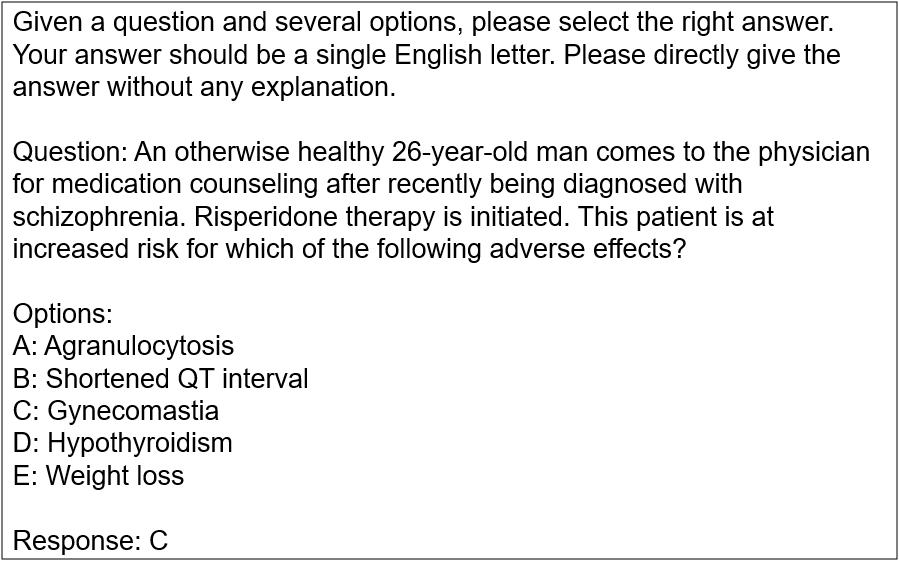
\includegraphics[width=0.45\textwidth]{Figure/Mental_Health_QA.png}
    \caption{Example for Mental Health QA}
    \label{fig: mental health QA}
\end{figure}

\subsubsection{Knowledge Tasks} We present a comprehensive performance analysis of various models on the QA task. Analyzing the results from the USMLE-mental dataset in \tabref{tab: USMLE-mental} and the results from the Crisis Response QA dataset in \tabref{tab: crisis response QA}, we draw several conclusions.

\paragraph{Lack of Mental Health Knowledge} GPT-4 emerges as the standout performer, demonstrating significantly superior performance in contrast to other models. Notably, \textbf{only GPT-4 achieved an average accuracy exceeding 60\%}, underscoring the formidable challenges inherent in mental health QA. The performance of models with smaller parameter sizes in these QA tasks closely aligns with the random baseline, accentuating a substantial performance gap when compared to their larger counterparts. It becomes evident that LLMs with smaller parameter sizes lack the comprehensive mental health knowledge base exhibited by models with larger parameter sizes. 

\paragraph{Foundational Knowledge vs. Clinical-Skill Knowledge} These models exhibit relatively superior proficiency in handling tasks falling under Step 1, emphasizing foundational scientific knowledge. However, their performance diminishes when confronted with tasks associated with Step 2, which involve more intricate clinical knowledge scenarios. The challenges presented in Step 2, leaning toward clinically relevant questions, introduce heightened complexity. This observed performance decrement in Step 2 suggests that the model \textbf{encounters difficulties when tasked with understanding and navigating the intricacies of real-world clinical scenarios}. The need for a more nuanced comprehension of clinical complexities, often encountered in diagnostic and therapeutic settings, becomes evident. Therefore, addressing the challenges presented in Step 2 becomes imperative for enhancing the model's applicability in clinical mental health contexts.

\paragraph{General Medical vs. Mental Health} Comparing GPT-3.5-turbo's performance on our dataset with its performance on full medical USMLE (Step1: 55.8\%, Step2: 59.1\%)~\citep{kung2023performance} exposes specific challenges and limitations in mental health queries. This indicates the unique challenges in the field of mental health compared to general medical domains.

\paragraph{Fine-tuned Models vs. General Models} MedAlpaca, fine-tuned on medical text using Alpaca as a base, outperforms Alpaca, indicating the efficacy of fine-tuning for enhancing mental health-related knowledge. Mental-LLaMA and Mental-Alpaca, fine-tuned for mental health prediction, show moderate improvement, with a limited extent. However, the performance of these three models on the Crisis Response QA dataset is concerning, exhibiting poorer results compared to their pre-fine-tuned counterparts.

\begin{table}[ht]
    \centering
    \footnotesize
    \begin{tabular}{l c c c c c c c c}
    \hline
    \textbf{Model} & \textbf{MH QA} & \textbf{Step1} & \textbf{Step2}\\
    \hline
    Random & 20.00 & 20.00 & 20.00\\
    \hline
    GPT-4 & \textbf{67.68} & \textbf{71.10} & \textbf{65.16}\\
    GPT-3.5-turbo & 45.12 & 49.68 & 41.77\\
    GPT-3.5-turbo-16k & 45.39 & 50.32 & 41.77\\
    \hline
    LLaMA2 & 25.44 & 26.73 & 23.88\\
    Alpaca & 24.76 & 25.97 & 23.87\\
    Vicuna-v1.5 & 23.38 & 23.38 & 23.39\\
    \hline
    Chinese-LLaMA2 & 20.08 & 23.05 & 17.90\\
    Chinese-Alpaca2 & 20.77 & 22.73 & 19.33\\
    ChatGLM2 & 20.77 & 23.05 & 19.09\\
    \hline
    MedAlpaca & 28.34 & 29.22 & 27.68\\
    Mental-Alpaca & 25.17 & 28.25 & 22.92\\
    MentalLLaMA & 25.58 & 27.27 & 24.34\\
    \hline
    \end{tabular}
    \caption{Models Performance on USMLE-mental dataset (Metrics: Accuracy 100\%). Step 1 primarily focuses on foundational knowledge, while Step 2 is clinical-skill oriented.}
    \label{tab: USMLE-mental}
\end{table}

\begin{table}[ht]
    \centering
    \footnotesize
    \begin{tabular}{l|c}
    \hline
    \textbf{Model} & \textbf{CR QA}\\
    \hline
    Random & 25.00\\
    \hline
    GPT-4 & \textbf{92.81}\\
    GPT-3.5-turbo & 88.24\\
    GPT-3.5-turbo-16k & 89.54\\
    \hline
    LLaMA2 & 77.78\\
    Alpaca & 56.21 \\
    Vicuna-v1.5 & 64.71\\
    \hline
    Chinese-LLaMA2 & 60.78\\
    Chinese-Alpaca2 & 63.40\\
    ChatGLM2 & 76.47\\
    \hline
    MedAlpaca & 53.59 \\
    Mental-Alpaca &  55.56 \\
    MentalLLaMA & 53.59 \\
    \hline
    \end{tabular}
    \caption{Models Performance on Crisis Response QA dataset (Metrics: Accuracy 100\%).}
    \label{tab: crisis response QA}
\end{table}


\subsubsection{Diagnostic Tasks} We extensively compared various models for the Diagnosis Prediction via Online Text Data and Simulated Doctor-Patient Dialogue tasks, as presented in\tabref{tab: SMHD} and \tabref{tab: D4}.%\KZ{Tables 4 and 5}.

In the diagnosis prediction via online text data, models demonstrated strong predictive capabilities for \textbf{depression and anxiety}, leveraging explicit symptoms in social media posts. However, predicting conditions like \textbf{bipolar disorder, schizophrenia, PTSD, autism} posed challenges due to higher ambiguity. For instance, bipolar disorder might be misdiagnosed as depression, and symptoms might not be readily expressed in textual content, as in the case of schizophrenia. 

\paragraph{Poor in Multiple Disorders Diagnosis} All models exhibited subpar performance in complex multiple disorder diagnoses, suggesting a limitation in their ability to handle intricate diagnostic tasks. This underscores the need for further improvements in the models' capacity to address multifaceted diagnostic challenges.

\paragraph{GPT-4 vs. GPT-3.5} In a longitudinal comparison of model performance, GPT-4's results were inferior to those of GPT-3.5-turbo and GPT-3.5-turbo-16k. Through error analysis, it was discovered that GPT-4 tends to be fixated on the `symptom-disease' process during disease diagnosis, often overlooking the potential mental states of posting users, as shown in Appendix \ref{app: model comparison}. It only correctly predicts when users explicitly manifest depressive symptoms in their posts, whereas GPT-3.5 is more accurate in such situations. In the diagnosis prediction via simulated doctor-patient dialogue data, GPT-4 also displayed an inclination toward the 'symptom-disease' process, often overlooking the actual states of patients, as shown in Appendix \ref{app: model comparison}.

\paragraph{Limitations of the Context Window} In this task, \textbf{models with a 2k context struggled}, impacting the performance of models like mental-Alpaca and mental-LLaMA, despite secondary training. Longer context window models, like GPT-3.5-turbo-16k, showed better performance. This highlights the importance of the context window in complex mental health diagnostic settings.

\begin{table*}[htbp]
\centering
\footnotesize
\begin{tabular}{l c c c c c c c c c c c}
\hline
\textbf{Model} & \textbf{Dep.} & \textbf{Anx.} & \textbf{Bip.} & \textbf{Sch.} & \textbf{Eating} & \textbf{PTSD} & \textbf{Autism} & \textbf{OCD} & \textbf{ADHD} & \textbf{Mul.}\\
\hline
GPT-4 & 42 & 66 & 42 & 42 & 30 & 36 & 34 & 30 & 62 & 22\\
GPT-3.5-turbo & 68 & \textbf{86} & 54 & 48 & 62 & 48 & 54 & 60 & 64 & 24\\
GPT-3.5-turbo-16k & \textbf{74} & \textbf{86} & \textbf{62} & \textbf{62} & \textbf{68} & \textbf{50} & \textbf{60} & \textbf{66} & \textbf{68} & \textbf{28}\\
\hline
LLaMa2 & 62 & 70 & 50 & 40 & 54 & 42 & 52 & 38 & 52 & 10\\
Alpaca & 24 & 36 & 28 & 14 & 12 & 18 & 26 & 20 & 24 & 6\\
Vicuna-v1.5 & 64 & 78 & 50 & 42 & 56 & 40 & 48 & 50 & 48 & 8\\
\hline
Chinese-LLaMA2 & 52 & 68 & 44 & 36 & 42 & 44 & 38 & 40 & 44 & 10\\
Chinese-Alpaca2 & 54 & 70 & 48 & 40 & 46 & 42 & 46 & 42 & 44 & 12\\
ChatGLM2 & 66 & 80 & 56 & 40 & 56 & 44 & 56 & 44 & 46 & 12\\
\hline
MedAlpaca & 20 & 34 & 24 & 12 & 8 & 12 & 16 & 12 & 18 & 4\\
Mental-Alpaca & 32 & 44 & 32 & 20 & 20 & 32 & 34 & 22 & 30 & 8\\
MentalLLaMA & 30 & 42 & 32 & 22 & 24 & 30 & 30 & 20 & 28 & 10\\
\hline
\end{tabular}
\caption{Models Performance on Diagnosis Prediction via Online Text Data (Metrics: Accuracy 100\%). "Dep." stands for depression, "Anx" stands for anxiety, "Bip." stands for bipolar, "Sch." stands for schizophrenia, and "Mul." stands for "multiple disorders". }
\label{tab: SMHD}
\end{table*}

\begin{table}[htpb]
\centering
\footnotesize
\begin{tabular}{l c c }
\hline
\textbf{Model} & \textbf{Depression} & \textbf{Suicide}\\
\hline
GPT-4 & 36.92 & \textbf{69.23}\\
GPT-3.5-turbo & 51.54 & 64.62\\
GPT-3.5-turbo-16k & \textbf{53.08} & 67.69\\
\hline
LLaMa2 & 16.15 & 10.77\\
Alpaca & 12.31 & 9.23\\
Vicuna-v1.5 & 15.38 & 15.38\\
\hline
Chinese-LLaMA2 & 22.31 & 20.00\\
Chinese-Alpaca2 & 24.62 & 21.54\\
ChatGLM2 & 23.08 & 20.77\\
\hline
MedAlpaca & 11.54 & 9.23\\
Mental-Alpaca & 19.23 & 12.31\\
MentalLLaMA & 19.23 & 17.69\\
\hline
\end{tabular}
\caption{Models Performance on Diagnosis Prediction via Dialogue (Metrics: Accuracy 100\%)}
\label{tab: D4}
\end{table}

\subsubsection{Emotional Support Tasks}
\paragraph{Automatic Evaluation} The automatic evaluation results are presented in \tabref{tab: automatic evaluation results}, where the BLEU metric requires the model's outputs, generated following the strategies outlined in the dataset, to be compared with responses provided by real-world mental health professionals in the dataset. Notably, GPT-3.5-turbo-16k achieved the highest BLEU score, indicating closer alignment with responses from mental health professionals. GPT-4, on the other hand, attained the highest D1 and D2 scores, reflecting greater text diversity. When compared to smaller models specifically trained for this task within PsyQA~\citep{sun-etal-2021-psyqa}, although LLMs exhibit lower BLEU scores, they demonstrate higher text diversity.

The models fine-tuned on Chinese data, namely Chinese-LLaMA2, Chinese-Alpaca2, and ChatGLM2, exhibited superior performance in this task when evaluated in the Chinese language context. However, the models that underwent fine-tuning for specific tasks, such as MedAlpaca, Mental-Alpaca, and MentalLLaMA, showed a degree of reduced generalization capability. This reduction occasionally manifested in empty outputs or repetitive responses in this task.

%We conducted a comprehensive comparison of various models in Therapeutic Tasks, and the results are presented in Table 6. In the Therapeutic Conversation task, after obtaining the model's output, we had \textbf{GPT-4 score the model's output based on the ground truth from 1 to 5}~\citep{liu2023geval}. GPT-4 demonstrated exceptional performance across all metrics, achieving the highest GPT4 score, Empathy ACC, and Safety ACC. 
%\KZ{How did you measure empathy ACC and safety ACC? These should have been explained in the task setup section.} 
%It's noteworthy that GPT-4, GPT-3.5-turbo, and GPT3.5-turbo-16k exhibited relatively similar performance. While GPT-4 showed advancements over GPT-3.5, it is conceivable that architectural improvements and parameter increases might not be substantial enough to significantly surpass GPT-3.5 in specific mental health therapeutic tasks. The additional complexity and parameters in GPT-4 may not have a pronounced impact on the nuanced differences in tasks related to mental health therapy, resulting in GPT-3.5 exhibiting similar performance. 

%However, it is crucial to highlight that the performance of all models, including GPT-4 and GPT-3.5-turbo, was \textbf{consistently subpar in these Therapeutic Tasks}. This observation prompts further investigation into the specific challenges posed by mental health therapeutic scenarios and underscores the need for model enhancements tailored to this domain. 

\begin{table}[htbp]
\centering
\footnotesize
\begin{tabular}{l c c c}
\hline
\textbf{Model} & \textbf{BLEU} & \textbf{D1} & \textbf{D2}\\
\hline
GPT-4 & 11.14 & \textbf{50.76} & \textbf{89.26}\\
GPT-3.5-turbo & 11.67 & 47.21 & 86.98\\
GPT-3.5-turbo-16k & \textbf{12.81} & 46.76 & 85.90\\
\hline
LLaMa2 & 6.84 & 42.73 & 74.53\\
Alpaca & 5.73 & 38.75 & 65.41\\
Vicuna-v1.5 & 7.62 & 42.57 & 70.13\\
\hline
Chinese-LLaMA2 & 10.12 & 42.36 & 73.68\\
Chinese-Alpaca2 & 12.13 & 41.95 & 74.53\\
ChatGLM2 & 10.68 & 47.60 & 83.98\\
\hline
MedAlpaca & 3.23 & 23.19 & 42.30\\
Mental-Alpaca & 4.82 & 24.61 & 46.32\\
MentalLLaMA & 4.55 & 26.15 & 44.35\\
\hline
\end{tabular}
\caption{Automatic evaluation results. The BLEU score is computed by averaging BLEU-1,2,3,4. All numerical values have been scaled up by a factor of one hundred.}
\label{tab: automatic evaluation results}
\end{table}

\paragraph{Human Evaluation vs. GPT4 Score} Subsequently, we considered the human evaluation metrics proposed by PsyQA~\citep{sun-etal-2021-psyqa}. We randomly selected 30 instances and the outputs of six models with relatively superior performance. GPT-4 and four human evaluators participated in the assessment. Fleiss' Kappa~\citep{fleiss1971measuring} was computed to measure the consistency between GPT-4 scores and human evaluator scores. The results exhibited good consistency on these metrics. Additionally, we integrated evaluation metrics proposed by EPITOME~\citep{sharma-etal-2020-computational} for assessing empathy in model outputs. Again, we randomly selected 30 instances and the outputs of the aforementioned six models. GPT-4 and four human evaluators were engaged in the evaluation process, and Fleiss' Kappa was computed to gauge the consistency between GPT-4 scores and human evaluator scores. The outcomes demonstrated good consistency, showed in \tabref{tab: consistency}. Generally, a kappa value above 0.6 is considered to indicate moderate consistency, but in the medical domain, a kappa value above 0.8 is deemed more acceptable~\citep{mchugh2012interrater}. Therefore, we will present both GPT-4 scores and human ratings for reference.

\begin{table*}[htbp]
\centering
\footnotesize
\begin{tabular}{l c c c c c c c}
\hline
\textbf{Model} & \textbf{Fluency} & \textbf{Coherence} & \textbf{Relevance} & \textbf{Helpfulness} & \textbf{Emo.} & \textbf{Int.} & \textbf{Exp.}\\
\hline
Fleiss' Kappa & 0.87 & 0.82 & 0.64 & 0.56 & 0.68 & 0.62 & 0.66\\
\hline
\end{tabular}
\caption{The consistency between GPT-4 scores and human evaluator scores. 'Emo.' stands for Emotional Reactions, 'Int.' stands for Interpretations and 'Exp.' stands for Explorations.}
\label{tab: consistency}
\end{table*}

\paragraph{Outstanding Fluency and Coherence} From \tabref{tab: PsyQA metrics gpt4} and \tabref{tab: PsyQA metrics human}, it can be observed that the best-performing LLM models in terms of Fluency and Coherence are comparable to human mental health counselors. Many models have approached the level of human counselors. Interestingly, in human evaluations, participants perceived that most LLMs exhibit higher relevance than human mental health counselors. However, this perception might be influenced by the models' tendency to repeat the seeker's questions. Moreover, participants perceived that models from the GPT series, were equally helpful as human mental health counselors, and in some instances, even more adept at addressing the issues raised by the seekers.

\begin{table}[htbp]
\centering
\footnotesize
\begin{tabular}{l c c c c}
\hline
\textbf{Model} & \textbf{Flu.} & \textbf{Coh.} & \textbf{Rel.} & \textbf{Help.}\\
\hline
Human & 2.90 & 2.73 & \textbf{2.76} & \textbf{2.47}\\
\hline
GPT-4 & - & - & - & -\\
GPT-3.5-turbo & 2.93 & 2.80 & 2.52 & 2.28\\
GPT-3.5-turbo-16k & \textbf{2.96} & \textbf{2.88} & 2.60 & 2.30\\
\hline
LLaMa2 & 2.65 & 2.52 & 2.31 & 1.96\\
Alpaca & 2.31 & 2.25 & 2.15 & 1.85\\
Vicuna-v1.5 & 2.67 & 2.43 & 2.25 & 1.86\\
\hline
Chinese-LLaMA2 & 2.89 & 2.26 & 2.28 & 2.05\\
Chinese-Alpaca2 & 2.90 & 2.59 & 2.40 & 2.10\\
ChatGLM2 & 2.96 & 2.75 & 2.52 & 2.26\\
\hline
MedAlpaca & 1.48 & 1.50 & 1.32 & 1.30\\
Mental-Alpaca & 1.50 & 1.42 & 1.40 & 1.33\\
MentalLLaMA & 1.55 & 1.53 & 1.44 & 1.35\\
\hline
\end{tabular}
\caption{Evaluation results under the PsyQA metrics~\citep{sun-etal-2021-psyqa} scored by \textbf{GPT-4}. 'Flu.' stands for fluency, 'Coh.' stands for coherence, 'Rel.' stands for relevance, 'Help.' stands for helpfulness}
\label{tab: PsyQA metrics gpt4}
\end{table}

\begin{table}[htbp]
\centering
\footnotesize
\begin{tabular}{l c c c c}
\hline
\textbf{Model} & \textbf{Flu.} & \textbf{Coh.} & \textbf{Rel.} & \textbf{Help.}\\
\hline
Human & 2.90 & 2.72 & 2.72 & 2.65\\
\hline
GPT-4 & 2.93 & 2.65 & 2.66 & 2.60\\
GPT-3.5-turbo & 2.93 & \textbf{2.73} & 2.75 & \textbf{2.68}\\
GPT-3.5-turbo-16k & \textbf{2.96} & \textbf{2.73} & \textbf{2.82} & 2.62\\
\hline
Vicuna-v1.5 & 2.66 & 2.55 & 2.50 & 2.03\\
Chinese-Alpaca2 & 2.72 & 2.73 & 2.73 & 2.25\\
ChatGLM2 & 2.82 & 2.64 & 2.75 & 2.40\\
\hline
\end{tabular}
\caption{Evaluation results under the PsyQA metrics~\citep{sun-etal-2021-psyqa} scored by \textbf{human}. 'Flu.' stands for fluency, 'Coh.' stands for coherence, 'Rel.' stands for relevance, 'Help.' stands for helpfulness}
\label{tab: PsyQA metrics human}
\end{table}

\paragraph{Lack of Empathy}However, the models demonstrated less favorable results in terms of empathy, as indicated in \tabref{tab: empathy metrics gpt4} and \tabref{tab: empathy metrics human}. Despite providing the models with specific response strategies and explicitly instructing them to exhibit empathy, the models struggled to consistently generate strong and effective Emotional Reactions, Interpretations, and Explorations. This highlights a notable limitation in the models' ability to consistently capture and convey empathetic responses in the context of mental health conversations, suggesting a need for further refinement in their understanding and expression of empathetic nuances.

\begin{table}[htbp]
\centering
\footnotesize
\begin{tabular}{l c c c}
\hline
\textbf{Model} & \textbf{Emo.} & \textbf{Int.} & \textbf{Exp.}\\
\hline
Human & \textbf{2.20} & \textbf{2.16} & \textbf{1.68}\\
\hline
GPT-4 & - & - & -\\
GPT-3.5-turbo & 1.84 & 1.66 & 1.58\\
GPT-3.5-turbo-16k & 2.02 & 1.64 & 1.60\\
\hline
LLaMa2 & 1.53 & 1.42 & 1.35\\
Alpaca & 1.42 & 1.50 & 1.34\\
Vicuna-v1.5 & 1.62 & 1.64 & 1.64\\
\hline
Chinese-LLaMA2 & 1.42 & 1.36 & 1.56\\
Chinese-Alpaca2 & 1.50 & 1.44 & 1.30\\
ChatGLM2 & 1.80 & 1.52 & 1.44\\
\hline
MedAlpaca & 1.14 & 1.16 & 1.20\\
Mental-Alpaca & 1.20 & 1.14 & 1.20\\
MentalLLaMA & 1.18 & 1.15 & 1.23\\
\hline
\end{tabular}
\caption{Empathy evaluation results scored by \textbf{GPT-4}. The metrics were proposed by EPITOME~\citep{sharma-etal-2020-computational}. 'Emo.' stands for Emotional Reactions, 'Int.' stands for Interpretations and 'Exp.' stands for Explorations.}
\label{tab: empathy metrics gpt4}
\end{table}

\begin{table}[htbp]
\centering
\footnotesize
\begin{tabular}{l c c c}
\hline
\textbf{Model} & \textbf{Emo.} & \textbf{Int.} & \textbf{Exp.}\\
\hline
Human & \textbf{2.05} & \textbf{1.82} & \textbf{1.57}\\
\hline
GPT-4 & 1.72 & 1.48 & 1.43\\
GPT-3.5-turbo & 1.63 & 1.50 & 1.40\\
GPT-3.5-turbo-16k & 1.88 & 1.55 & 1.40\\
\hline
Vicuna-v1.5 & 1.60 & 1.50 & 1.50\\
Chinese-Alpaca2 & 1.51 & 1.43 & 1.28\\
ChatGLM2 & 1.78 & 1.33 & 1.42\\
\hline
\end{tabular}
\caption{Empathy evaluation results scored by \textbf{human}. The metrics were proposed by EPITOME~\citep{sharma-etal-2020-computational} and scored by GPT4. 'Emo.' stands for Emotional Reactions, 'Int.' stands for Interpretations and 'Exp.' stands for Explorations.}
\label{tab: empathy metrics human}
\end{table}

\paragraph{Safe Outputs} Regarding the models' performance in ensuring output safety showed in \tabref{tab: safety metrics}, while some models occasionally exhibited empty responses or repetitive phrases, most model outputs consistently demonstrated high safety standards. The provided information was accurate, conducive to offering mental health support, easy to comprehend, and free from apparent or implicit verbal violence. Moreover, the outputs had no discernible adverse physical or psychological effects on the seeker. However, it is worth noting that in some instances, the models responded with seemingly plausible but potentially inaccurate information. Despite this occasional drawback, the overall safety of the outputs remained commendable, emphasizing the models' responsible behavior in mental health counseling scenarios.

\begin{table}[htbp]
\centering
\footnotesize
\begin{tabular}{l c}
\hline
\textbf{Model} & \textbf{Safety Rank}\\
\hline
Human & \textbf{6.84}\\
\hline
GPT-4 & 6.62\\
GPT-3.5-turbo & 6.56\\
GPT-3.5-turbo-16k & 6.60\\
\hline
LLaMa2 & 5.32\\
Alpaca & 5.16\\
Vicuna-v1.5 & 5.44\\
\hline
Chinese-LLaMA2 & 6.02\\
Chinese-Alpaca2 & 6.10\\
ChatGLM2 & 6.35\\
\hline
MedAlpaca & 2.60\\
Mental-Alpaca & 2.84\\
MentalLLaMA & 2.88\\
\hline
\end{tabular}
\caption{Safety evaluation results scored by \textbf{fine-tuned BERT-base}. The metrics and evaluator were proposed by Dialogue Safety~\citep{qiu2023benchmark}. 'Emo.' stands for Emotional Reactions, 'Int.' stands for Interpretations and 'Exp.' stands for Explorations.}
\label{tab: safety metrics}
\end{table}

%\begin{table}[htbp]
%\centering
%\footnotesize
%\begin{tabular}{l c c c}
%\hline
%\textbf{Model} & \textbf{Response} & \textbf{Empathy} & \textbf{Safety}\\
%\hline
%GPT-4 & \textbf{4.20} & \textbf{46.92} & \textbf{48.28}\\
%GPT-3.5-turbo & 3.66 & 44.62 & 39.90\\
%GPT-3.5-turbo-16k & 3.82 & 46.15 & 42.36\\
%\hline
%LLaMa2 & 2.05 & 25.38 & 19.70\\
%Alpaca & 1.84 & 15.38 & 14.78\\
%Vicuna-v1.5 & 1.92 & 27.69 & 19.21\\
%\hline
%Chinese-LLaMA2 & 2.75 & 27.69 & 25.61\\
%Chinese-Alpaca2 & 2.94 & 30.77 & 29.06\\
%ChatGLM2 & 2.81 & 26.15 & 28.57\\
%\hline
%MedAlpaca & 1.63 & 13.84 & 12.32\\
%Mental-Alpaca & 1.72 & 14.61 & 12.32\\
%MentalLLaMA & 1.80 & 16.15 & 13.30\\
%\hline
%\end{tabular}
%\caption{Models Performance on Therapeutic Tasks. The metric for Generated Response is GPT4 score. The metrics for Empathy and Safety are Accuracy 100\%.}
%\end{table}